\subsection{OpenCL}
The project requires interaction with heterogeneous processing devices present within a user's system.
It achieves this via the hardware vendor's implementation of the \ac{OpenCL} library.

\ac{OpenCL} is an open framework for executing tasks, described by C99-syntax \emph{kernels}, on a variety of devices.
Suitable targets include a range of heterogeneous devices such as multi-core \acp{CPU}, \acp{APU}, and \ac{GPU} from the majority of commodity hardware vendors.

The Khronos Group maintains and frequently updates the \ac{OpenCL} standard\cite{khronos}.
Participating vendors include \ac{AMD}, Apple, Intel, and NVIDIA \textemdash{} although the quality and accessibility of implementations varies greatly.

A stated goal of the \ac{OpenCL} project is to ``allow cross-platform parallel programming''.
The underlying processing devices present on a system are abstracted, allowing code to be written without explicit knowledge of target architectures.
This theoretically enables developers to write applications for a person system and then later scale execution to a massively parallel workstation, without significant code modification.

\begin{figure}[h]
\begin{center}
	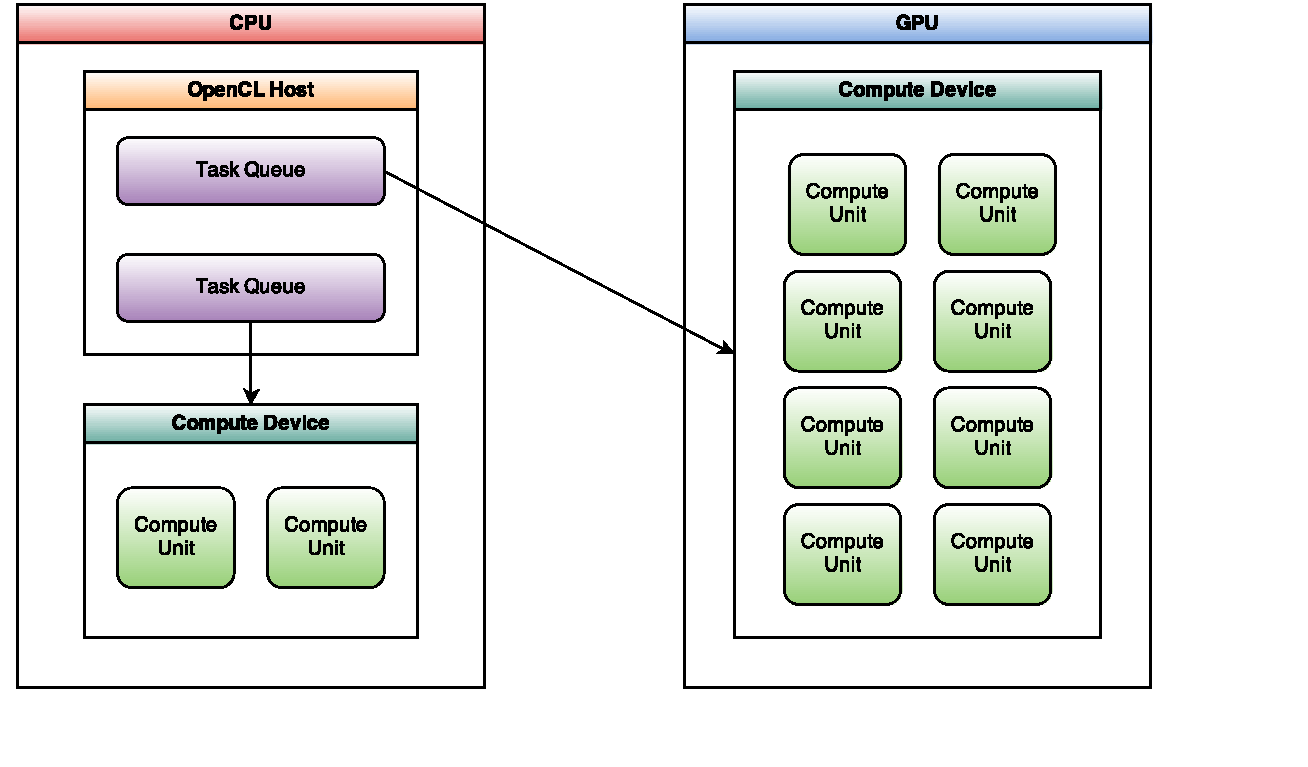
\includegraphics[width=4.8in]{./figures/OpenCLModel}
	\captionof{figure}{The OpenCL architecture model.}
	\label{fig:ocl_model}
\end{center}
\end{figure}

\paragraph{Architecture model}
As Figure~\ref{fig:ocl_model} illustrates, the architecture model presented by \ac{OpenCL} is as follows:

\begin{description}
\item[Host device] The system's \ac{CPU}. It interacts with an execution environment, responsible for discovering and selecting compute devices present on the system. The host device initialises one or more \emph{contexts}, whereby any devices within a single context have access to shared task and memory buffers.

\item[Compute devices] The system's available processing devices, capable of scheduling \ac{OpenCL} kernel work-groups. Before enumerating compute devices, the available \emph{platforms} must be discovered by the runtime. Usually, there is a platform presented for each unique \ac{OpenCL} supporting vendor with hardware installed. Devices are then retrieved on a per-platform bases, either filtered by type (\ac{CPU}/\ac{GPU}) or not.

\item[Compute Units] Discrete units of hardware present within a processing devices, capable of scheduling and executing \ac{OpenCL} kernel instances.
Kernel execution occurs across internal \emph{processing units}, such as \acp{ALU}.
\end{description}

\begin{figure}[h]
	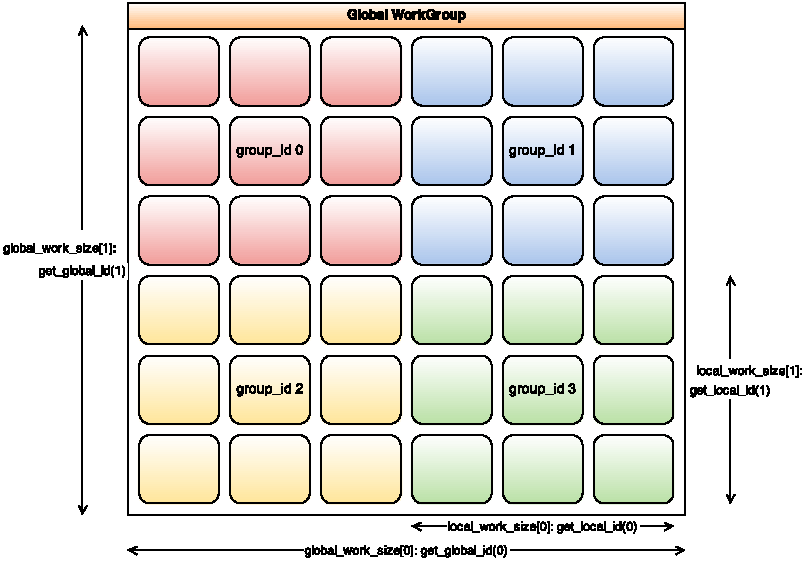
\includegraphics[width=4.8in]{./figures/workgroups}
	\captionof{figure}{The OpenCL execution model.}
	\label{fig:ocl_ex_model}
\end{figure}

\paragraph{Execution Model}
\ac{OpenCL} has a simple execution model, allowing both \emph{coarse-grained} and \emph{fine-grained} parallelism. Programmers write parallel code from the reference frame of a single kernel execution. Each instance orients itself only via access to its \emph{local} and \emph{global} \verb|id|, expanded on shortly. Larger calculations are a direct result of cooperating kernel instances. 

Kernel instances, scheduled for execution on compute devices, as referred to as \emph{work-items}.

The \ac{OpenCL} standard calls a collection of work-items a \emph{work-group}. Work-groups are the unit of work dispatched to a device. The number of work-items within a group that a device should schedule is set by the programmer, providing the \verb|global_work_size| parameter. Each kernel invocation is enumerated with a global \verb|id|. 

In addition to flat enumeration, the computation can benefit from the abstraction of work \emph{dimensions}. For example, a calculation over $100$ elements can represented as a 2-dimensional $10 \times 10$ calculation. When utilising dimensional abstraction, access to either unique global \verb|id| or $x, y$ offsets is available.

Higher dimensions are available for further structuring of tasks. It is clear that the spatial abstraction provided when there is a topological significant within the processed data. In these circumstances, the \verb|local_work_size| parameter provides further benefits.

When \verb|local_work_size| is specified, again possibly with dimensionality, the work-items are additionally divided into subgroups. Memory allocation can use the \verb|__local| qualifier. In this case, data will reside in higher-bandwidth buffers that can only be synchronised between members of the same local work-group. With the addition of this second, local tier of memory, the \ac{OpenCL} model hints at how efficient kernels should be constructed. Being aware of the positioning of data and its dependencies is key to developing efficient kernels, free of memory-synchronisation bottlenecks.

Much of the project's implementation effort concerning \ac{OpenCL} will be mapping data required by common algorithms to efficient arrangements within device memory. This mirrors \ac{OpenCL} development in general.
The fact that this task is so laborious is a reason why heterogeneous parallel programming is still under-utilised in the wild.

\paragraph{Comparison with CUDA}
\ac{OpenCL} is not the only computation framework choice when interacting with \ac{GPGPU} devices. As mentioned earlier, a competing technology is NVIDIA's \ac{CUDA}.

During the planning phase, RubiCL considered both choices. Ultimately, the decision was made to use \ac{OpenCL} over \ac{CUDA} for several major reasons:

\begin{description}
  \item[Multiple vendor support]
    \ac{CUDA} is not an open standard. Its parallelism framework is only available on NVIDIA hardware. Using a library supported only by a single vendor to provide the project's hardware interfacing would lead to far fewer systems being able to benefit from accelerated processing.

  \item[CPU and GPGU execution]
    By using \ac{OpenCL}, RubiCL will be able to execute kernels on both \ac{CPU} and \ac{GPGPU} devices. This contrasts the \ac{GPGPU}-only focus of \ac{CUDA}.
    This greatly increases development convenience. Development can occur on a mobile laptop, functionally tested with its \ac{CPU}. Afterwards, the library will be transferred to desktop workstations for performance testing on a variety of hardware.

    In addition, this opens up the possibility of attempting code execution on both devices concurrently. This will investigate whether complete system-wide utilisation is beneficial for a single computation.
  \end{description}

  \paragraph{Disadvantages of choosing \ac{OpenCL}}
  There are several downsides to using \ac{OpenCL} instead of \ac{CUDA}. The programming model is generally agreed to be less developer friendly. This is perhaps due to the need to include far more abstraction over the range of target devices. In addition, due to the need for compatibility with several device families, \ac{OpenCL} can be less performant out-of-the-box than \ac{CUDA}. Advanced knowledge of how to tweak device-specific parameters to avoid execution bottlenecks can help avoid this.

  \paragraph{Current state of OpenCL implementations}
  A final major disadvantage of \ac{OpenCL} at the moment, is the current quality of some vendor implementations. All vendors advertise themselves as being \ac{OpenCL}-compatible when marketing their hardware. However, in reality it is harder than advertised to achieve a working system.

  For example, NVIDIA, have made no attempt to hide the fact that they would much rather everybody used \ac{CUDA} instead. They are so slow at releasing libraries that they are a full version of the \ac{OpenCL} specification behind other vendors at the time of writing this report. Features that are supported also perform much worse than expected.

  Intel are up-to-date with library implementations but only have non-Windows support if you have purchased non-consumer grade \emph{Xeon} processors.

  Hopefully these issues will be rectified if \ac{OpenCL} continues to gain tracking in future. As a short term response, the RubyCL project has been implemented on well-supported hardware only: An Apple Macbook Air containing a Intel Haswell processor, and a desktop system containing an \ac{AMD} \ac{CPU} and \ac{GPU}.

  Apple and \ac{AMD} both have high-quality \ac{OpenCL} $1.2$ libraries and seem to be the two companies most invested in increased \ac{OpenCL} uptake. Apple have recently started encouraging desktop software developer to schedule suitable tasks on the \ac{GPU} via OS X's \ac{GCD}.
